\begin{frame}{Amazon}
    \begin{columns}[c]
        \column{.4\textwidth}
        \begin{figure}
            \centering
            
\includegraphics[height=0.40\textheight]{images/Lumberyard_Logo.png}
            \caption{AWS Lumberyard logo \cite{AWS_Lumberyard_logo}}
            \label{fig:AWS_Lumberyard}
        \end{figure}
        \column{.6\textwidth}
        \begin{figure}
            \centering
            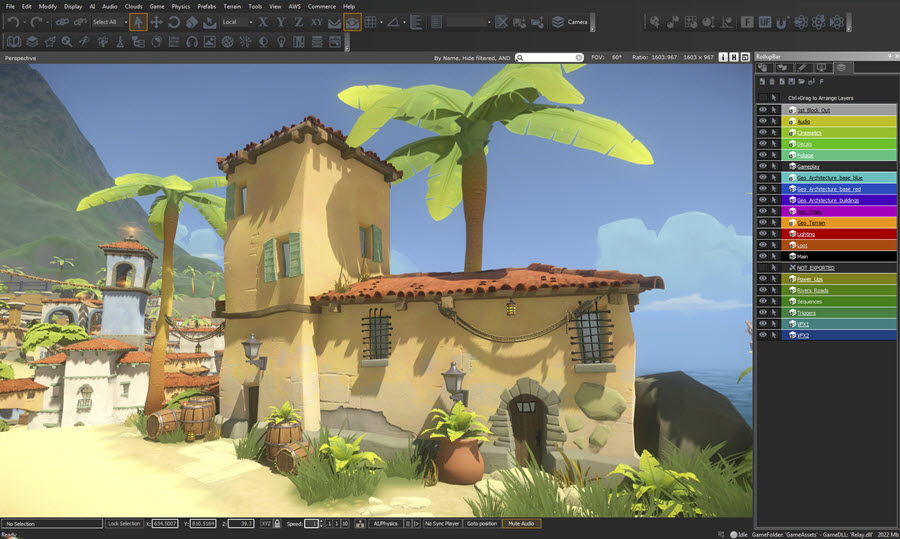
\includegraphics[height=0.60\textheight]{images/lumberyard_editor_relay_1.jpg}
            \caption{AWS Lumberyard widok \cite{AWS_Lumberyard_view}}
            \label{fig:social-media}
        \end{figure}
    \end{columns}
\end{frame}
    

\begin{frame}{Amazon}
    \begin{block}{Ograniczenia wykorzystania narzędzi AWS:}
        \emph{The terms state that Lumberyard is not to be used with drones, medical equipment, nuclear facilities, manned spacecraft or live military combat in normal times, but have a special exception.}   
    \end{block}  
    \pause
    \begin{block}{Zabezpieczenie na wypadek apokalipsy zombie:}
        \emph{Clause 57.10 of the AWS terms of service states: “This restriction will not apply in the event of the occurrence (certified by the United States Centers for Disease Control or successor body) 
        of a widespread viral infection transmitted via bites or contact with bodily fluids that causes human corpses to reanimate and seek to consume living human flesh, blood, brain or nerve tissue and is 
        likely to result in the fall of organised civilisation.”} \cite{GUARDIAN_AWS_ZOMBIE}   
    \end{block}      
\end{frame}

\begin{frame}{Gamestation}
    SOULS \cite{Soul_EULA}     
\end{frame}

    
    